\documentclass{beamer}
\usepackage[utf8]{inputenc}
\usepackage{graphicx}
\usepackage{hhline}
\usepackage{pdfpages}
\usepackage{xcolor}
\usepackage{makecell}
\usepackage[mode=buildnew]{standalone}
\usepackage{amsmath}
\usepackage{mathtools}
\usepackage{tikz}
\usepackage{environ}
\usepackage{fontawesome}
\usepackage{caption}
\usepackage[backend=bibtex,style=authoryear-comp,dashed=false,natbib=true]{biblatex}
\addbibresource{bibtex.bib}
% \setbeamertemplate{footline}[frame number]
\graphicspath{{img/}}
\setbeamertemplate{navigation symbols}{}
\setbeamertemplate{page number in head/foot}{}
\setbeamertemplate{bibliography item}{}
\setbeamertemplate{caption}[numbered]
\setbeamercovered{transparent}
\renewcommand\refname{Bibliography}
\setbeamerfont{institute}{size=\small}
\usetheme{Frankfurt}
\usecolortheme{whale}
\DeclareMathOperator*{\argmax}{argmax} 
\DeclareCaptionFormat{myformat}{\fontsize{5}{6}\selectfont#1#2#3}
\captionsetup{format=myformat}
\captionsetup[figure]{labelfont={bf},name={Fig.},labelsep=period}
\captionsetup[table]{labelfont={bf},name={Table}}

\newcommand{\customframefont}[1]{
	\setbeamertemplate{itemize/enumerate body begin}{#1}
	\setbeamertemplate{itemize/enumerate subbody begin}{#1}
}

\NewEnviron{framefont}[1]{
	\customframefont{#1} % for itemize/enumerate
	{#1 % For the text outside itemize/enumerate
		\BODY
	}
	\customframefont{\normalsize}
}

\setbeamertemplate{footline}{% 
	\hfill% 
	\usebeamercolor[fg]{page number in head/foot}% 
	\usebeamerfont{page number in head/foot}% 
	\insertframenumber%
	%\,/\,\inserttotalframenumber
	\kern1.2em\vskip4.5pt% 
}

\renewcommand\cellgape{\Gape[3pt]}
\definecolor{ao(english)}{rgb}{0.0, 0.5, 0.0}

\title{Supervised Spam Classification}
\subtitle{``Comparing Effectivity and Robustness of Sequential and Non-Sequential Machine-Learning Models"}
\author{Atreya Shankar, Cognitive Systems (M.Sc.)}
\institute{BM2: Intelligent Data Analysis (IDA) \\ University of Potsdam, SoSe 2019 \\ Prof. Dr. Tobias Scheffer}
\date{August 08. 2019}

\begin{document}
	\begin{frame}
		\maketitle
	\end{frame}
	
	\begin{frame}
		\frametitle{Table of Contents}
		\setbeamertemplate{enumerate items}[square]
		\begin{enumerate}
			\setlength\itemsep{1em}
			\item Introduction
			\item Methodologies
			\item Results
			\item Evaluation
			\item Conclusions
			\item Bibliography
		\end{enumerate}
	\end{frame}
	
	\section{Introduction}
	\subsection{}
	\begin{framefont}{\footnotesize}
		\begin{frame}
			\frametitle{Introduction}
			\vspace{-10pt}
			\begin{columns}
				\column{0.003\linewidth}
				\column{0.40\linewidth}
				\centering
				\begin{figure}
					\captionsetup{justification=centering}
					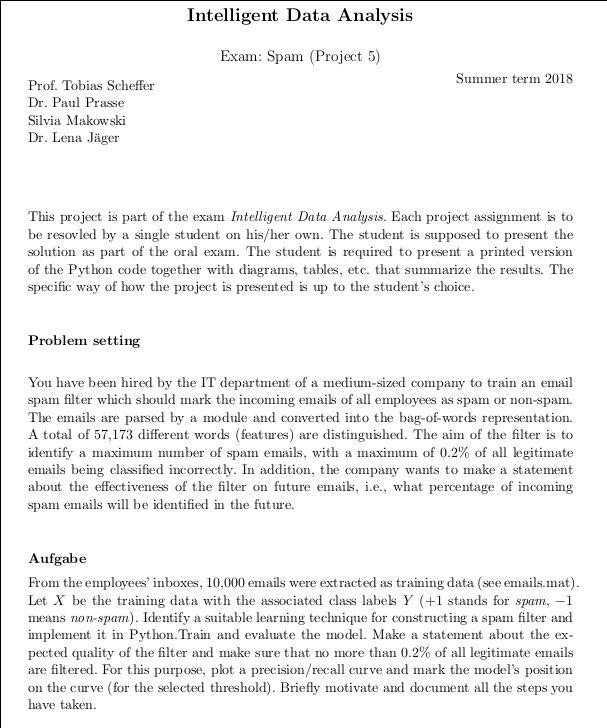
\includegraphics[trim={0.5cm 0cm 0.5cm 0.2cm},clip,width=4.7cm]{project_description.png}
					\caption{Spam project description}
				\end{figure}
				\column{0.60\linewidth}
				\begin{itemize}
					\setlength\itemsep{1.5em}
					\item Project description proposes using data in ``emails.mat" file with 10k instances and $\sim$50k features
					\item Bag-of-words form of data, which would only work for non-sequential learning
					\item Enron-spam pre-processed text data derived from Enron Corporation scandal; subset of employees' emails became publicly available \parencite{metsis2006spam}
					\item Consists of 33,716 text-based emails; 16,545 ``ham" and 17,171 spam instances
				\end{itemize}
			\end{columns}
		\end{frame}
	\end{framefont}
	
	\subsection{}
	\begin{framefont}{\footnotesize}
		\begin{frame}
			\frametitle{Objectives}
			\begin{itemize}
				\setlength\itemsep{1.5em}
				\item Utilize enron-spam emails database to implement both sequential and non-sequential supervised classifiers
				\item Meet project requirement to develop a classifier that attains 99.8\% recall on ``ham" emails
				\item Provide input into recall values for future spam emails given selected optimal threshold
				\item Additionally, provide insights into effectivity and robustness of sequential and non-sequential models
			\end{itemize}
		\end{frame}
	\end{framefont}
	
	\section{Methodologies}
	\begin{framefont}{\footnotesize}
		\begin{frame}
			\frametitle{Overview}
			\vspace{-10pt}
			\begin{columns}
				\column{0.003\linewidth}
				\column{0.40\linewidth}
				\centering
				\begin{figure}
					\captionsetup{justification=centering}
					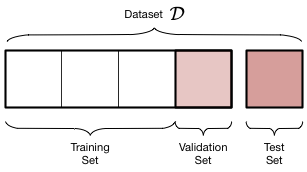
\includegraphics[width=4.3cm]{train-validate-test.png}
					\caption{Data splitting schematic \parencite{split}}
				\end{figure}
				\column{0.60\linewidth}
				\begin{itemize}
					\setlength\itemsep{1.5em}
					\item Non-sequential model: Support Vector Machine (SVM)
					\item Sequential model: CNN-LSTM with word/character embeddings
					\item Due to time limitations, K-fold cross-validation was omitted
					\item Compromise: train/validate/test on the same subsets of data for fair comparison
					\item (Train $\cup$ Validation):Test $\Longrightarrow$ 70:30
					\item Train:Validation $\Longrightarrow$ 85:15	
			\end{itemize}
			\end{columns}
		\end{frame}
	\end{framefont}
	
\begin{framefont}{\footnotesize}
	\begin{frame}
		\frametitle{Non-Sequential Model: Support Vector Machine (SVM)}
		\vspace{-10pt}
		\begin{columns}
			\column{0.003\linewidth}
			\column{0.40\linewidth}
			\centering
			\begin{figure}
				\captionsetup{justification=centering}
				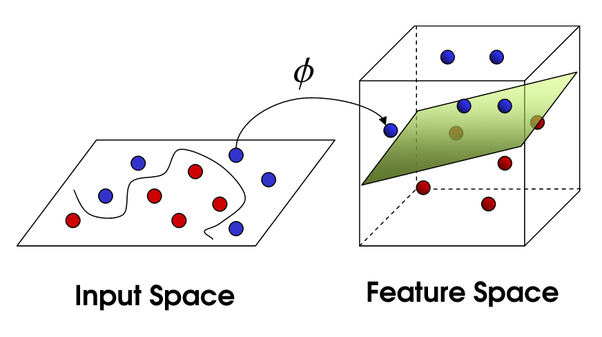
\includegraphics[width=4.3cm]{svm.png}
				\caption{Support Vector Machine (SVM) schematic \parencite{svmSchematic}}
			\end{figure}
			\column{0.60\linewidth}
			\begin{itemize}
				\setlength\itemsep{1.5em}
				\item Pre-processing text to normalized bag-of-words representation with $|V| = 5,000$ words
				\item Sklearn's \texttt{SGDClassifier} with Mini-Batch SGD and early stopping
				\item Linear and approximated RBF Kernel \texttt{(RBFSampler)}
				\item Grid-search over batch-size, regularization term $\alpha$, RBF kernel $\gamma$, and number of sampling components for \texttt{RBFSampler}
			\end{itemize}
		\end{columns}
	\end{frame}
\end{framefont}

\begin{framefont}{\footnotesize}
	\begin{frame}
		\frametitle{Sequential Model: CNN-LSTM (Words)}
		\vspace{-10pt}
		\begin{columns}
			\column{0.003\linewidth}
			\column{0.40\linewidth}
			\centering
			\begin{figure}
				\captionsetup{justification=centering}
				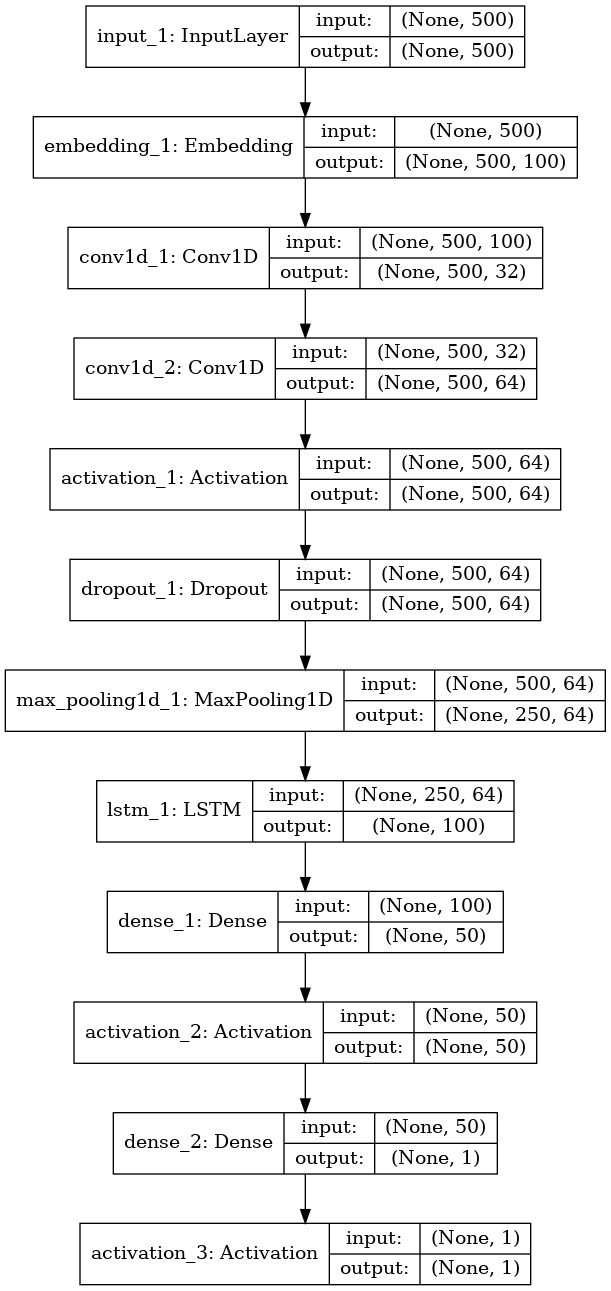
\includegraphics[width=3cm]{model.png}
				\caption{Keras schematic for CNN-LSTM (Words)}
			\end{figure}
			\column{0.60\linewidth}
			\begin{itemize}
				\setlength\itemsep{1.5em}
				\item Pre-processing text to padded/clipped integer encoded tokens with $|V| = 5,000$ words
				\item 1-dimensional CNN with varying filters to enrich sequential features; LSTM cell to capture short and long-term sequential relationships; dropout regularization for model robustness
				\item Grid-search over embedding dimensions, dropout rate, batch-size and learning rate
				\item Learning both with and without pre-trained GloVe word vectors ($\sim$6 billion tokens)
			\end{itemize}
		\end{columns}
	\end{frame}
\end{framefont}

\begin{framefont}{\footnotesize}
	\begin{frame}
		\frametitle{Sequential Model: CNN-LSTM (Words+Characters)}
		\vspace{-10pt}
		\begin{columns}
			\column{0.003\linewidth}
			\column{0.40\linewidth}
			\centering
			\begin{figure}
				\captionsetup{justification=centering}
				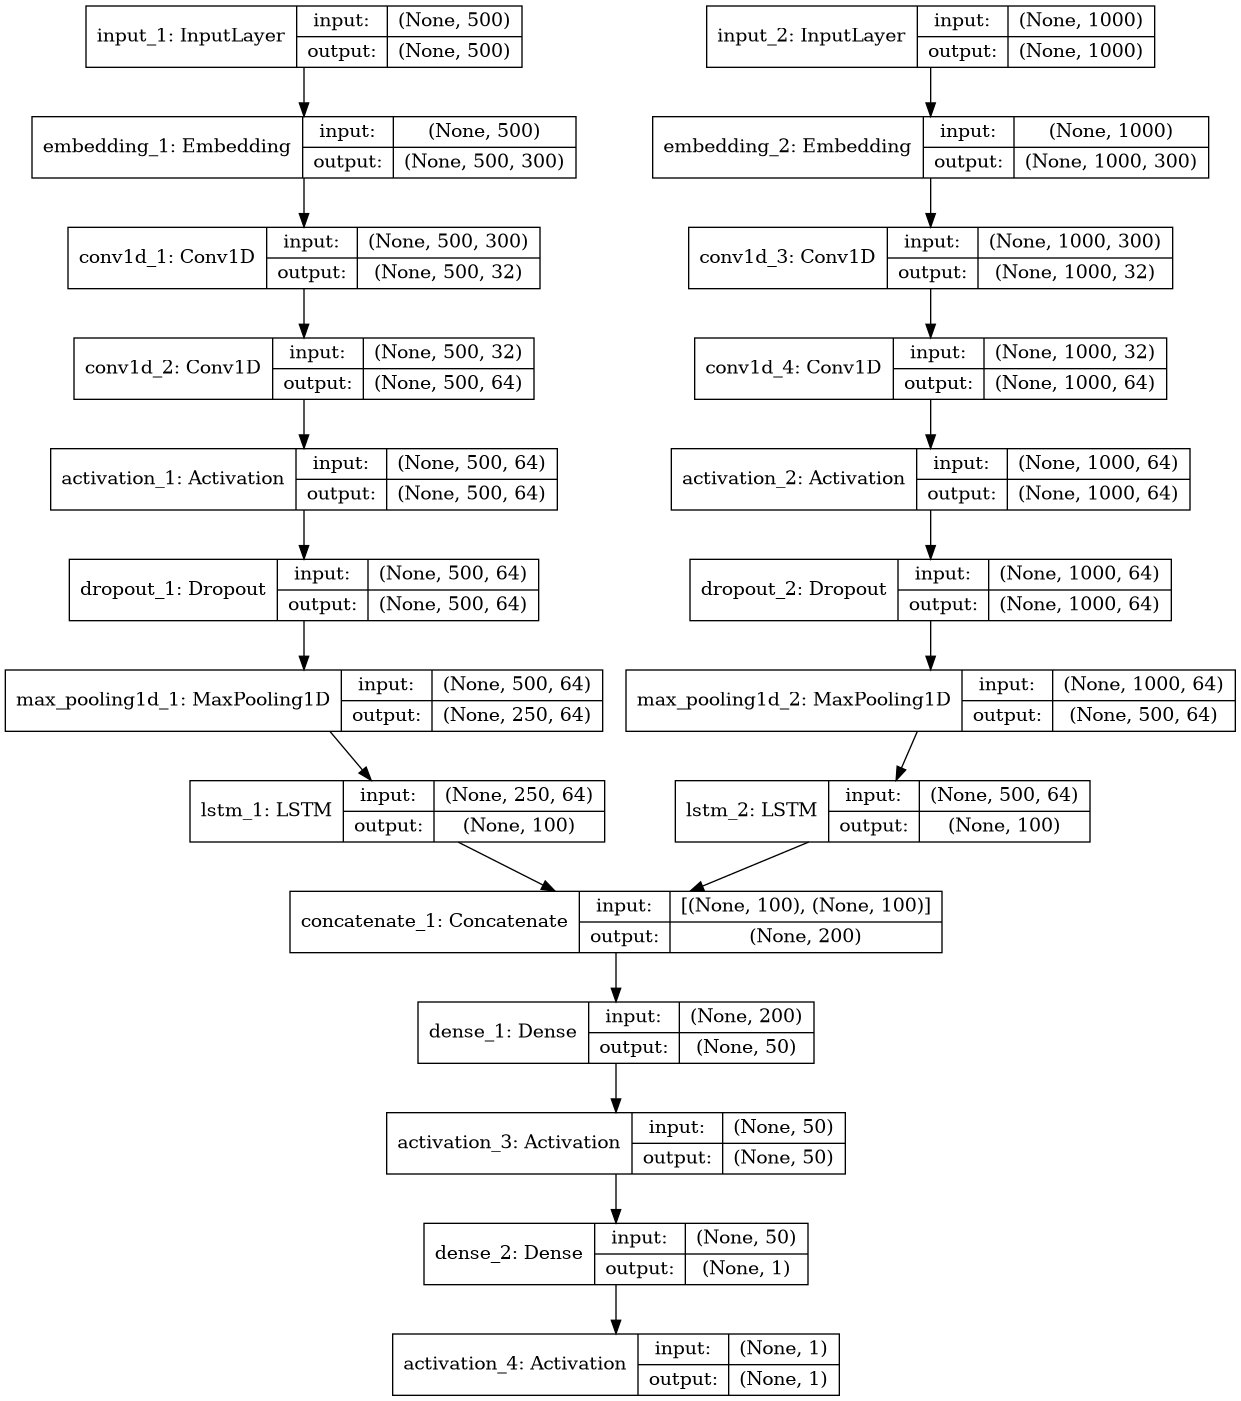
\includegraphics[width=4.6cm]{model_combined.png}
				\caption{Keras schematic for CNN-LSTM (Words+Characters)}
			\end{figure}
			\column{0.60\linewidth}
			\begin{itemize}
				\setlength\itemsep{1.5em}
				\item Using character sequences to overcome unknown token issue; same general architecture as before
				\item Grid-search over embedding dimensions, dropout rate, batch-size and learning rate
				\item Learning both with and without pre-trained GloVe word vectors ($\sim$6 billion tokens)
				\item Approximating GloVe character embeddings by averaging over character-containing word vectors \parencite{charEmbed}
			\end{itemize}
		\end{columns}
	\end{frame}
\end{framefont}

\section{Results}
\subsection{}
\begin{framefont}{\footnotesize}
	\begin{frame}
		\frametitle{Grid-search optimal models}
		\begin{table}
			\centering
			\captionsetup{justification=centering}
			\bgroup
			\def\arraystretch{1.5}
			\begin{tabular}{|c|c|c|} \hline
				Classifier & Test F$_1$ & ROC-AUC \\ \hhline{|=|=|=|}
				SVM (Linear Kernel) & 0.9836 & \textbf{0.9965} \\ \hline
				SVM (Approximated RBF Kernel) & 0.3437 & 0.4063 \\ \hline
				CNN-LSTM (Words) & 0.9753 & 0.9972 \\ \hline
				CNN-LSTM (Words+Characters) & 0.9808 & 0.9975 \\ \hline
				\makecell{CNN-LSTM \\(Words+GloVe)} & 0.9902 & \textbf{0.9989} \\ \hline 
				\makecell{CNN-LSTM \\(Words+Characters+GloVe)} & 0.9902 & \textbf{0.9989} \\ \hline
			\end{tabular}
			\egroup
			\caption{Summary of grid-search optimal models; zero rule classifier baseline is 50.9\%; F$_1$ scores with fixed threshold at 0 and 0.5 for SVM and CNN-LSTM respectively}
		\end{table}
		\vspace{-10pt}
		\begin{itemize}
			\item Both sequential and non-sequential models achieve high F$_1$ and ROC-AUC test scores
		\end{itemize}
	\end{frame}
\end{framefont}

\subsection{}
\begin{framefont}{\footnotesize}
	\begin{frame}
		\frametitle{``Ham" Relative Importance Analysis (SVM)}
		\centering
		\begin{figure}
			\captionsetup{justification=centering}
			\includegraphics[width=10.5cm]{ham_words.pdf}
			\caption{Relative importance analysis for SVM (linear kernel)}
		\end{figure}
	\end{frame}
\end{framefont}

\subsection{}
\begin{framefont}{\footnotesize}
	\begin{frame}
		\frametitle{Spam Relative Importance Analysis (SVM)}
		\centering
		\begin{figure}
			\captionsetup{justification=centering}
			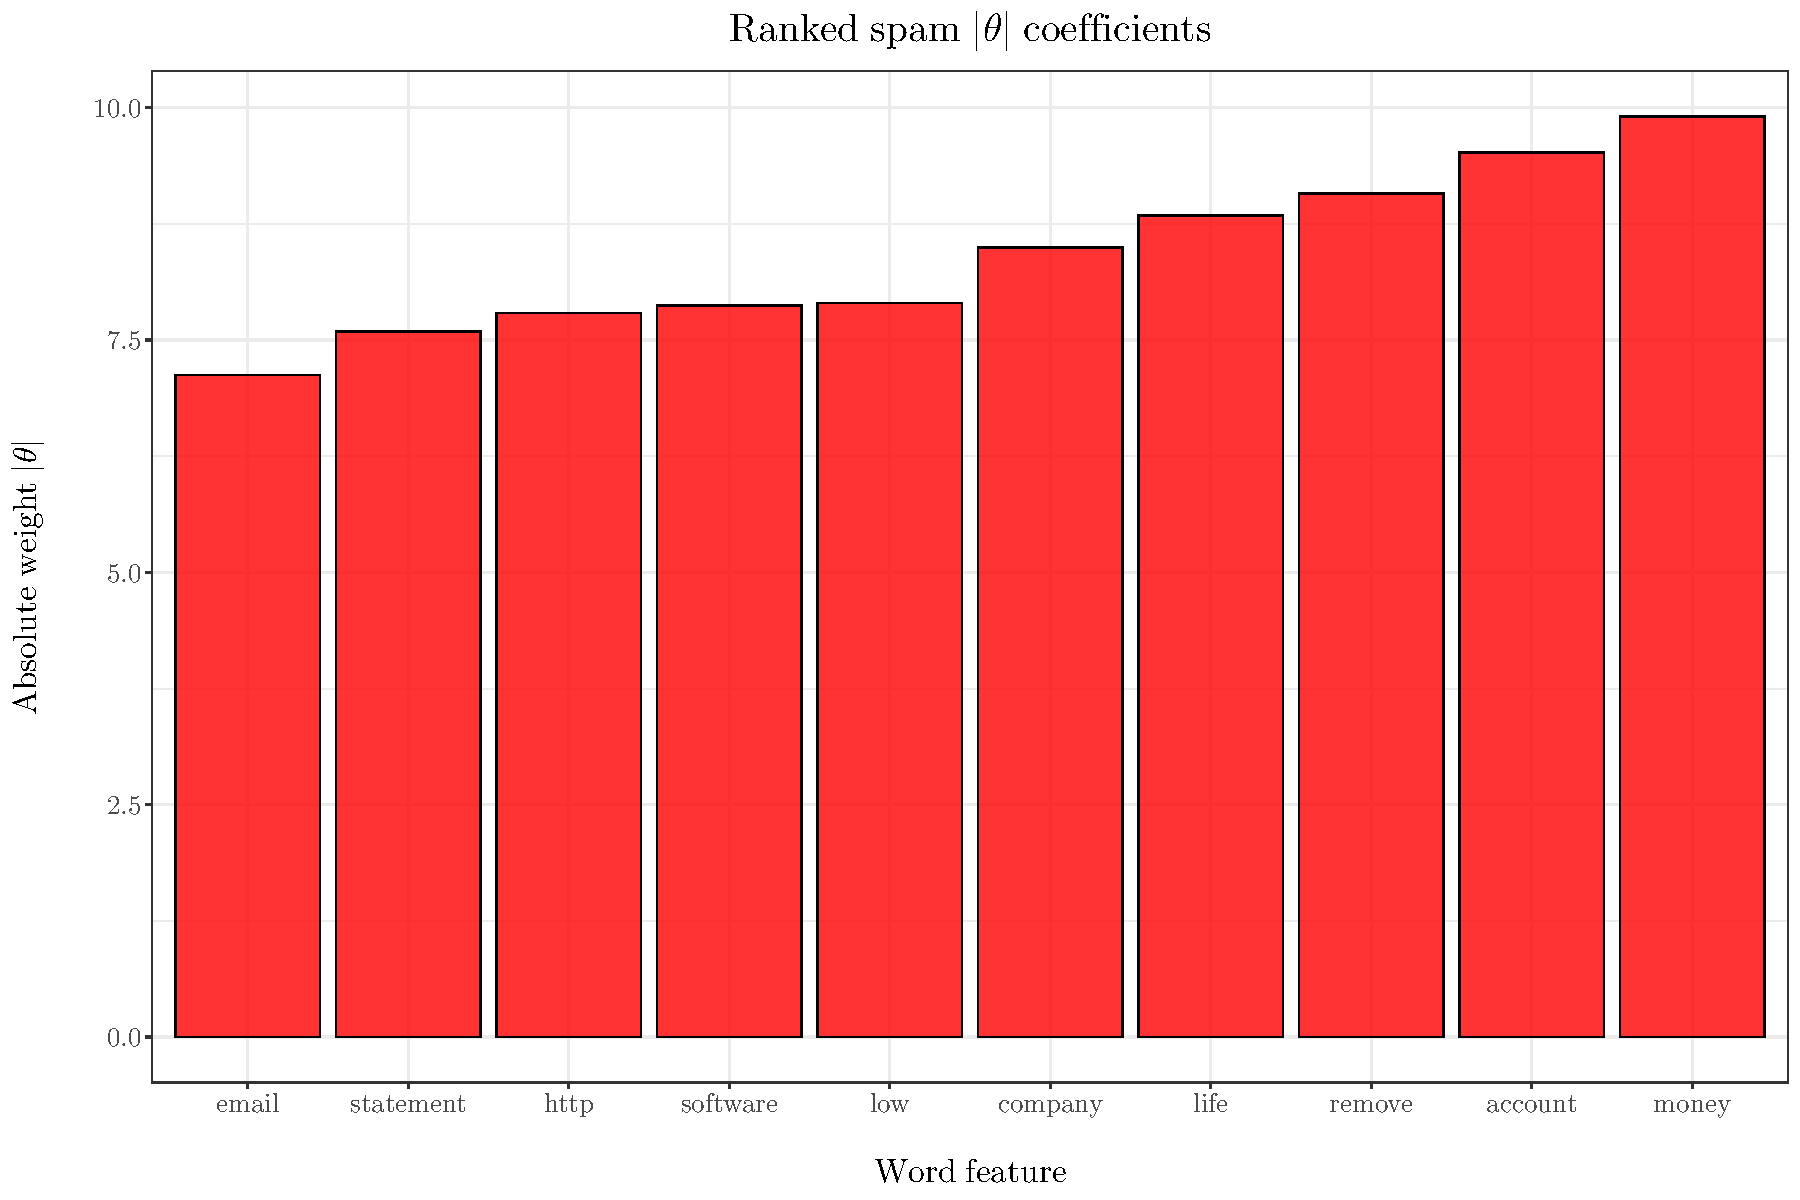
\includegraphics[width=10.5cm]{spam_words.pdf}
			\caption{Relative importance analysis for SVM (linear kernel)}
		\end{figure}
	\end{frame}
\end{framefont}

\section{Evaluation}
\subsection{}
\begin{framefont}{\footnotesize}
	\begin{frame}
		\frametitle{Optimal Threshold Analysis}
		\centering
		\begin{figure}
			\captionsetup{justification=centering}
			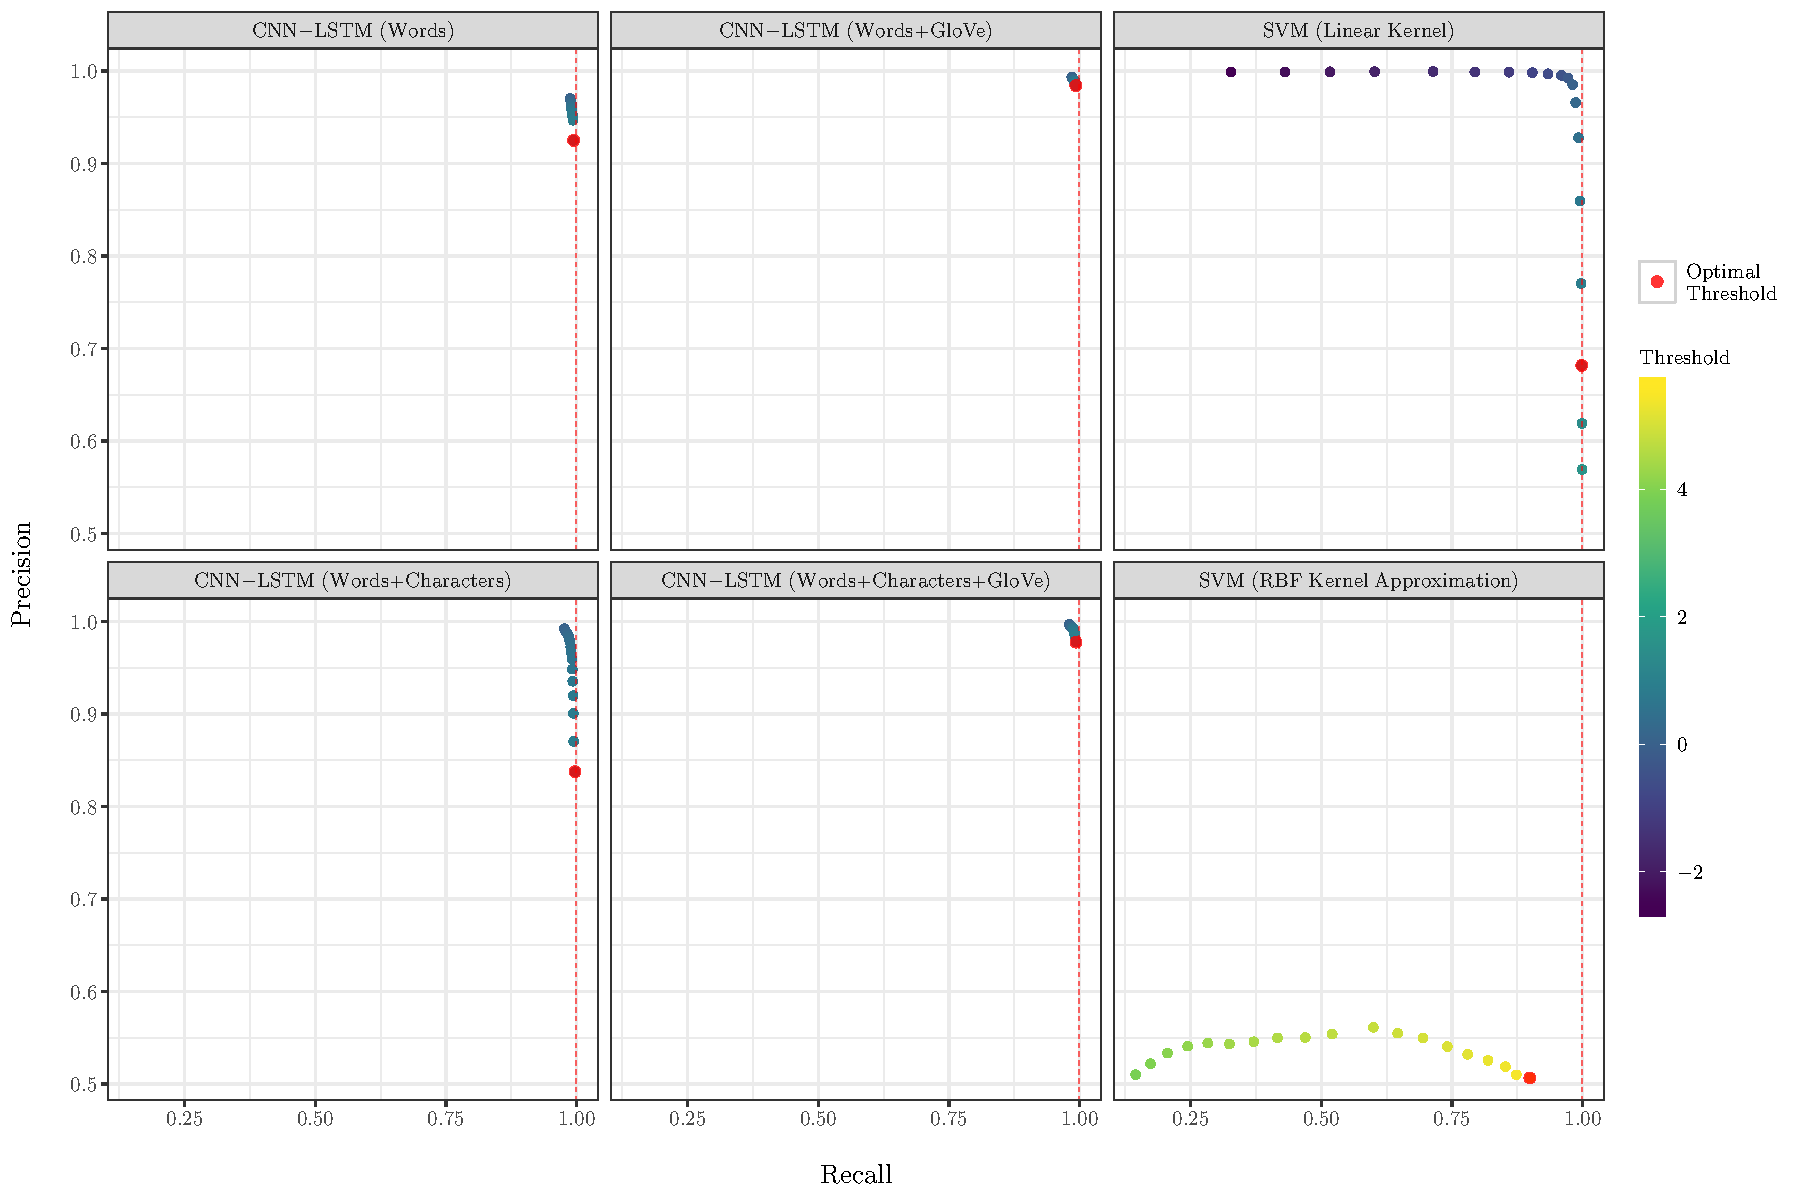
\includegraphics[trim={0cm 0cm 0.2cm 0cm},clip,width=11.2cm]{combined.pdf}
			\caption{Precision-Recall curve (ham label) for optimal threshold analysis}
		\end{figure}
	\end{frame}
\end{framefont}

\subsection{}
\begin{framefont}{\footnotesize}
	\begin{frame}
		\frametitle{Optimal Threshold Performance}
		\begin{table}
			\centering
			\bgroup
			\def\arraystretch{1.5}
			\begin{tabular}{|c|c|c|c|} \hline
				Classifier & Threshold & Recall $\lbrack$Spam$\rbrack$ & Recall $\lbrack$Ham$\rbrack$ \\ \hhline{|=|=|=|=|}
				SVM (Linear Kernel) & 1.171 & \color{red} 0.5509 & \textbf{0.9982} \\ \hline
				SVM (Approximated RBF Kernel) & 5.552 & 0.1558 & 0.8991 \\ \hline
				CNN-LSTM (Words) & 0.9444 & 0.9224 & 0.9943 \\ \hline
				CNN-LSTM (Words+Characters) & 0.9444  & \color{red} 0.8137 &  \textbf{0.9971} \\ \hline
				\makecell{CNN-LSTM \\(Words+GloVe)} & 0.9444  & \color{ao(english)} 0.9846  & \textbf{0.9929} \\ \hline
				\makecell{CNN-LSTM \\(Words+Characters+GloVe)} & 0.9444 & \color{ao(english)} 0.9781 & \textbf{0.9930} \\ \hline
			\end{tabular}
			\egroup
			\caption{Results of optimal threshold analysis}
		\end{table}
		\vspace{-10pt}
		\begin{itemize}
			\item Trade off between ham and spam recall; either accept low recall for spam or compromise with lower recall for ham
		\end{itemize}
	\end{frame}
\end{framefont}

\subsection{}
\begin{framefont}{\footnotesize}
	\begin{frame}
		\frametitle{Blind Dataset Performance (SMS Spam)}
		\begin{table}
			\centering
			\captionsetup{justification=centering}
			\bgroup
			\def\arraystretch{1.5}
			\begin{tabular}{|c|c|c|} \hline
				Classifier & Blind F$_1$ & ROC-AUC\\ \hhline{|=|=|=|}
				SVM (Linear Kernel) & 0.4688 & \textbf{0.7039} \\ \hline
				SVM (Approximated RBF Kernel) & 0.1785 & 0.4937 \\ \hline
				CNN-LSTM (Words) & 0.5090 & 0.6158 \\ \hline
				CNN-LSTM (Words+Characters) & 0.4416 & 0.6522 \\ \hline
				\makecell{CNN-LSTM \\(Words+GloVe)} & 0.2913 & \textbf{0.7567} \\ \hline
				\makecell{CNN-LSTM \\(Words+Characters+GloVe)} & 0.3017 & \textbf{0.7578} \\ \hline
			\end{tabular}
			\egroup
			\caption{Results of blind data test; zero rule classifier obtains 87\% due to class imbalance; F$_1$ scores with fixed threshold at 0 and 0.5 for SVM and CNN-LSTM respectivel}
		\end{table}
		\vspace{-10pt}
		\begin{itemize}
			\item Words-based models perform consistently well on blind dataset (albeit worse than zero rule classifier)
			\item Considering sequential nature of data contributes to some robustness
		\end{itemize}
	\end{frame}
\end{framefont}

\section{Conclusions}
\subsection{}
\begin{framefont}{\footnotesize}
	\begin{frame}
		\frametitle{Conclusions}
		\begin{itemize}
			\setlength\itemsep{1.2em}
			\item For spam detection, both sequential and non-sequential models are effective
			\item Trade-off exists between ``ham" and spam recall; an informed decision must be made
			\item Both words-based sequential and non-sequential models tend to be robust to new datasets; although sequential models tend to carry richer and more discriminating features
			\item High cost of training CNN-LSTM; perhaps not economical for a company to deploy GPU on IMAP server
			\item \textbf{SVM would be a more efficient and scalable option}
		\end{itemize}
	\end{frame}
\end{framefont}

\subsection{}
\begin{framefont}{\footnotesize}
	\begin{frame}
		\frametitle{Improvements to Embeddings in CNN-LSTM}
		\vspace{-10pt}
		\begin{columns}
			\column{0.003\linewidth}
			\column{0.40\linewidth}
			\centering
			\begin{figure}
				\captionsetup{justification=centering}
				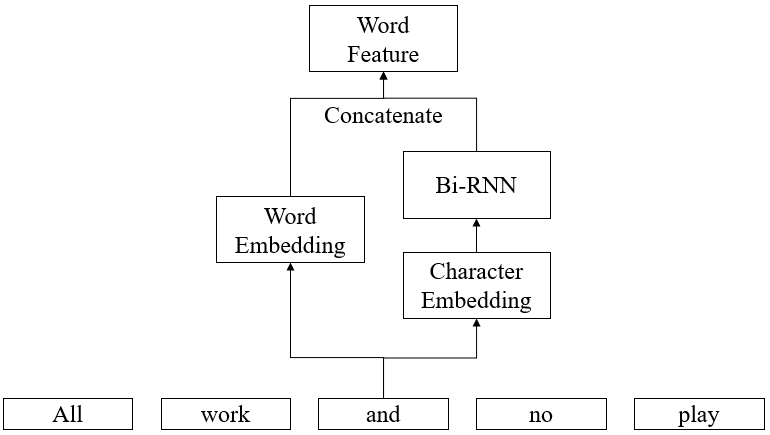
\includegraphics[width=4.5cm]{improved_rnn.png}
				\caption{Improved word-character embedding model \parencite{improvedRNN}}
			\end{figure}
			\column{0.60\linewidth}
			\begin{itemize}
				\setlength\itemsep{1.5em}
				\item Separate pipeline for character sequences leads to symbolic overfitting on types of datasets
				\item Can overcome unknown tokens but contributes uncertainty in terms of dialects and expressions
				\item \textcite{improvedRNN} proposes a bidirectional LSTM to enrich word vector features
				\item This could address the unknown token issue without leading to overfitting on entire character sequences
			\end{itemize}
		\end{columns}
	\end{frame}
\end{framefont}

\begin{frame}[allowframebreaks]
	\frametitle{Bibliography}
	\nocite{*}
	\printbibliography[title = {Bibliography}]
\end{frame}

\end{document}